\documentclass[11pt]{article}

\usepackage[margin=1in]{geometry}
\usepackage{amsmath}
\usepackage{booktabs}
\usepackage{graphicx}
\usepackage{hyperref}
\usepackage{url}

\graphicspath{{figures/}}

\title{Cost-Matched Diagnostics for Human-in-the-Loop Robot Learning Intervention Triggers}
\author{FORESIGHT-HIL Manuscript Draft}
\date{July 2, 2026}

\begin{document}

\maketitle

\begin{abstract}
Human-in-the-loop reinforcement learning can improve robot learning by injecting corrective actions when autonomous exploration is unsafe, slow, or unproductive. However, claims about intervention-trigger quality depend strongly on how human cost, checkpoint variance, and budget timing are measured. This paper frames FORESIGHT-HIL as a diagnostic evaluation protocol rather than as a current trigger-superiority claim. In a robosuite manipulation case study, an initially plausible learning-value trigger is overturned by cost matching: a lower-budget random baseline reaches higher repeated success at lower realized human-step cost than LV-VoI scale3. Two lightweight trigger repairs remain dominated, and intervention traces show that the failure is not simply a far-from-object querying problem. The contribution is a reproducible automation-science protocol for stress-testing HIL-RL trigger claims with cost-matched random families, repeated checkpoint evaluation, and trace-level budget diagnostics before expanding new trigger designs.
\end{abstract}

\section*{Note to Practitioners}
This paper is motivated by robot-learning workflows in which human corrections are useful but expensive. The practical lesson is that an intervention trigger should not be accepted because it beats one arbitrary random budget or one favorable checkpoint. Before a learned trigger is deployed, scaled to more tasks, or used to justify human-efficiency claims, practitioners should sweep random intervention budgets around the trigger's realized human-step cost, evaluate selected checkpoints repeatedly, inspect when interventions start, and stop a trigger variant when same-seed random baselines dominate it in both success and cost. The present experiments use a scripted privileged-state oracle in simulation rather than real teleoperators, so the numerical results should be read as a reproducible evaluation gate, not as a direct measurement of human workload. The accompanying artifact structure exposes the evidence registry, exact command templates, registry-generated tables, and trace fields needed to reproduce the diagnostic before adapting it to real users or hardware.

\section{Introduction}

Human-in-the-loop reinforcement learning (HIL-RL) is attractive for robotic manipulation because human interventions can redirect an agent away from unsafe, unproductive, or low-value exploration while adding corrective data to the learning process. Recent robot-learning systems combine interventions, demonstrations, and off-policy updates to improve sample efficiency in manipulation settings \cite{luo2025hilserl,ball2023rlpd}. More broadly, surveys of human involvement in learning systems emphasize that the human can shape development, training, evaluation, and deployment rather than merely supply an initial dataset \cite{retzlaff2024hitl}. In this setting, intervention timing is not only a control-design problem. It is a human-attention allocation problem: the trigger decides when a scarce, costly, and potentially safety-critical human resource is spent.

This allocation view changes what must be measured. A learned trigger can look human-efficient if it is compared with a single random baseline whose budget is too high or too low. A checkpoint can look strong if it is selected from a noisy training curve and evaluated only once. A trigger score can appear meaningful at the episode level while still spending budget at the wrong training phase or with poor calibration. These failure modes matter for robotics because real corrections carry opportunity cost, operator delay, interface burden, and safety implications. An intervention policy that merely moves cost into poorly measured parts of training is not yet evidence of better human-attention allocation.

FORESIGHT-HIL began from a method-positive hypothesis: a learning-value value-of-information trigger might request human help more efficiently than random intervention. The current evidence does not support that hypothesis. In the Lift case study, the LV-VoI scale3 trigger initially appeared plausible when compared with a higher-cost random baseline, but a random-budget sweep changed the conclusion. The cost-matched random b350 baseline reached 439/500 repeated successes (87.8\%) at 177.0 best-step human steps, while LV-VoI scale3 reached 416/500 repeated successes (83.2\%) at 202.0 human steps. Under the current evidence registry, the learned trigger is therefore dominated rather than Pareto-superior.

The paper turns this reversal into a diagnostic protocol for human-attention allocation claims in HIL-RL. The protocol asks whether a trigger survives three validity gates: random baselines swept around the trigger's realized human cost, repeated checkpoint evaluation with binomial uncertainty, and trace-level diagnostics of when and where interventions start. These checks are deliberately modest. They do not require a new robot platform or a full benchmark suite, but they do require enough measurement discipline to prevent an allocation claim from resting on a mismatched budget, a lucky checkpoint, or an uninterpreted aggregate success rate.

The resulting contribution is bounded but useful for automation science. We present a robotic manipulation case study in robosuite \cite{robosuite2020} using an SAC-style off-policy learner \cite{haarnoja2018sac,sac2018applications} and a scripted privileged-state oracle as the simulated intervention source. We show that cost matching reverses the apparent LV-VoI advantage, that two lightweight repairs remain dominated by same-seed random baselines, and that intervention traces point to budget-control and score-timing mismatch rather than a simple far-from-object failure. The paper therefore does not claim that the current LV-VoI trigger is superior. Its claim is that HIL-RL trigger papers should pass cost-matched, repeated-evaluation, and trace-level diagnostic gates before presenting intervention timing as a human-efficient improvement.

\section{Related Work}

HIL-RL and intervention learning have developed around the practical need to learn manipulation policies with fewer unsafe or low-value interactions. HIL-SERL-style systems combine human interventions with off-policy reinforcement learning and offline data, while RLPD shows how offline data can be mixed with online updates for efficient learning \cite{luo2025hilserl,ball2023rlpd}. Demonstration-learning infrastructure such as robomimic provides a complementary view of what matters when using human demonstration data for robot manipulation \cite{mandlekar2021robomimic}. These works motivate the learning backbone used here, but they do not by themselves settle how to evaluate a trigger that allocates human attention during training.

Interactive imitation learning and robot-gated correction study related querying problems. ThriftyDAgger treats expert queries as budgeted and gates them by novelty and risk, while adaptive intervention mechanisms can reduce takeover cost in robot-gated imitation learning \cite{hoque2021thrifty,cai2025aim}. Those systems are important baselines for the idea that a robot can decide when to ask, but the current paper studies a different diagnostic question: whether an HIL-RL intervention trigger remains convincing as an attention-allocation policy after cost-matched random baselines and repeated checkpoint estimates.

Model-based and calibration literature informs the diagnostic interpretation. PETS and MBPO motivate uncertainty-aware short rollouts and caution about when learned models should be trusted \cite{chua2018pets,janner2019mbpo}. Calibration work shows that neural-network confidence scores can be miscalibrated, which is directly relevant when a trigger score is used to spend a scarce human budget \cite{guo2017calibration}. Deep RL evaluation studies further warn that small numbers of seeds and point estimates can support unstable conclusions, motivating interval estimates and more careful reporting \cite{henderson2018deeprlmatters,agarwal2021statisticalprecipice}. The present work combines these concerns into an evaluation protocol for intervention-trigger claims that are really claims about human-attention allocation.

\section{Diagnostic Protocol and Experimental Setup}

The diagnostic protocol treats an intervention-trigger claim as a cost-sensitive human-attention allocation claim rather than as a simple learned-trigger-versus-random comparison. A trigger is not credited for being selective merely because its nominal budget differs from the baseline budget; it must be compared with random intervention policies whose realized human-step costs bracket the learned trigger. A trigger is also not credited from a single favorable checkpoint; selected checkpoints must be evaluated with repeated episodes and reported with uncertainty. Finally, aggregate success and cost are not sufficient when a trigger fails, because they do not explain how attention was spent. The protocol therefore combines cost-matched random families, repeated checkpoint evaluation, and trace-level intervention diagnostics as three validity gates.

The first validity gate is cost matching. Cost matching is performed against realized best-step human cost, not only against the nominal intervention budget assigned at launch. For each learned trigger under test, the random family is swept across nearby budgets so that at least one random point falls below and one falls near or above the trigger's realized cost when feasible. This converts the comparison from "learned trigger versus a random baseline" into a local success-cost frontier. In the Lift case study, this step is decisive: the lower-budget random b350 condition dominates LV-VoI scale3, so the protocol rejects the trigger-superiority interpretation before any repair is expanded.

The second validity gate is repeated checkpoint evaluation. This gate reduces dependence on a single final policy or a single restored-best evaluation. For paper-facing Lift claims, selected checkpoints are evaluated with repeated rollouts and reported as success counts, success proportions, Wilson confidence intervals, and realized human-step cost. Wilson intervals are used because they behave more reliably than simple normal approximations for finite binomial samples, especially near high success rates \cite{wilson1927score}. The protocol also keeps best-step and final-policy accounting separate so that a policy's apparent success is not confused with late training collapse or checkpoint-selection noise.

The third validity gate is trace-level diagnosis. Trace diagnostics are used after a trigger fails a cost-matched comparison because a dominated aggregate result does not reveal whether the trigger spent attention too early, too often, in the wrong geometry, or under miscalibrated scores. Each intervention start records the training step, the fraction of budget already spent, gripper-to-cube geometry, end-effector and object height, trigger score, and predicted failure probability when those quantities are available. These traces make mechanism hypotheses testable. For example, R023 shows that LV-VoI does not simply fail by asking far from the cube; it starts closer to the cube than random on average while spending many more intervention starts. R024 then shows that suppressing some low-score mid-run starts is mechanically possible but insufficient to recover the success-cost frontier.

The current case study uses robosuite Lift and Stack as simulated robotic manipulation environments \cite{robosuite2020}. The learner follows an off-policy SAC-style setup \cite{haarnoja2018sac,sac2018applications} with demonstration and intervention data motivated by offline-to-online robot learning and demonstration-learning practice \cite{ball2023rlpd,mandlekar2021robomimic}. The evaluated intervention strategies include no intervention, a random-budget family, LV-VoI scale3, a minimum-disagreement LV-VoI repair, and a score-floor LV-VoI repair. Lift supplies the main cost-matched diagnostic evidence; Stack is retained as boundary evidence showing that the current intervention mechanism does not yet transfer as a positive method result.

The intervention source is a scripted privileged-state oracle, not a real teleoperator. This design makes intervention timing reproducible and cheap enough to diagnose across seeds, budgets, and checkpoints, but it limits claims about real human workload, interface latency, fatigue, and embodiment transfer. Accordingly, all numerical claims in this paper are routed through the evidence registry and registry-generated R036 tables rather than copied manually from raw logs. Table~\ref{tab:protocol_checklist} summarizes the reporting gates that follow from this diagnostic setup.

\begin{table*}[t]
\centering
\caption{Diagnostic protocol checklist for HIL-RL intervention-trigger claims. Each gate is motivated by a failure mode surfaced in the Lift/Stack case study.}
\label{tab:protocol_checklist}
\begin{tabular}{p{0.07\textwidth}p{0.19\textwidth}p{0.32\textwidth}p{0.33\textwidth}}
\toprule
Gate & Requirement & What to report & Why it matters \\
\midrule
G1 & Cost-matched random family & At least one random budget below and above the method's realized human cost; report realized best-step human cost, not only nominal budget. & Prevents a learned trigger from appearing efficient only because the random baseline was mismatched. \\
G2 & Repeated checkpoint evaluation & Evaluate selected checkpoints with repeated episodes; report binomial confidence intervals and seed variability. & Single restored or final evaluations can change rankings in noisy RL settings. \\
G3 & Best-step and final-policy accounting & Report raw final policy, restored best policy, and best-step human cost. & Separates late collapse/checkpoint selection from true intervention efficiency. \\
G4 & Trace-level intervention diagnostics & Log intervention starts with timing, budget fraction, task geometry, score, and p\_fail when available. & Explains how a trigger spends budget and tests mechanism hypotheses. \\
G5 & Same-seed stop gate & Before expanding a repaired trigger, compare it against same-seed cost-matched random using repeated evaluation. & Stops weak heuristic repairs before expensive expansion and prevents over-tuning. \\
\bottomrule
\end{tabular}
\end{table*}


\section{Results}

The main result is a reversal under cost matching. In the initial five-seed reliability check, LV-VoI scale3 appeared plausible because it achieved a success rate close to a higher-cost random baseline. That interpretation changed once the random family was swept around the method's realized human cost. As shown in Table~\ref{tab:registry_costmatched_claims}, random b350 achieved 439/500 repeated successes (87.8\%, 95\% CI [84.6, 90.4]) at 177.0 best-step human steps, whereas LV-VoI scale3 achieved 416/500 repeated successes (83.2\%, 95\% CI [79.7, 86.2]) at 202.0 best-step human steps. The learned trigger is therefore not on the observed Lift success-cost frontier, so the current evidence does not support a claim that it allocates human attention more efficiently than random intervention.

\begin{figure*}[t]
    \centering
    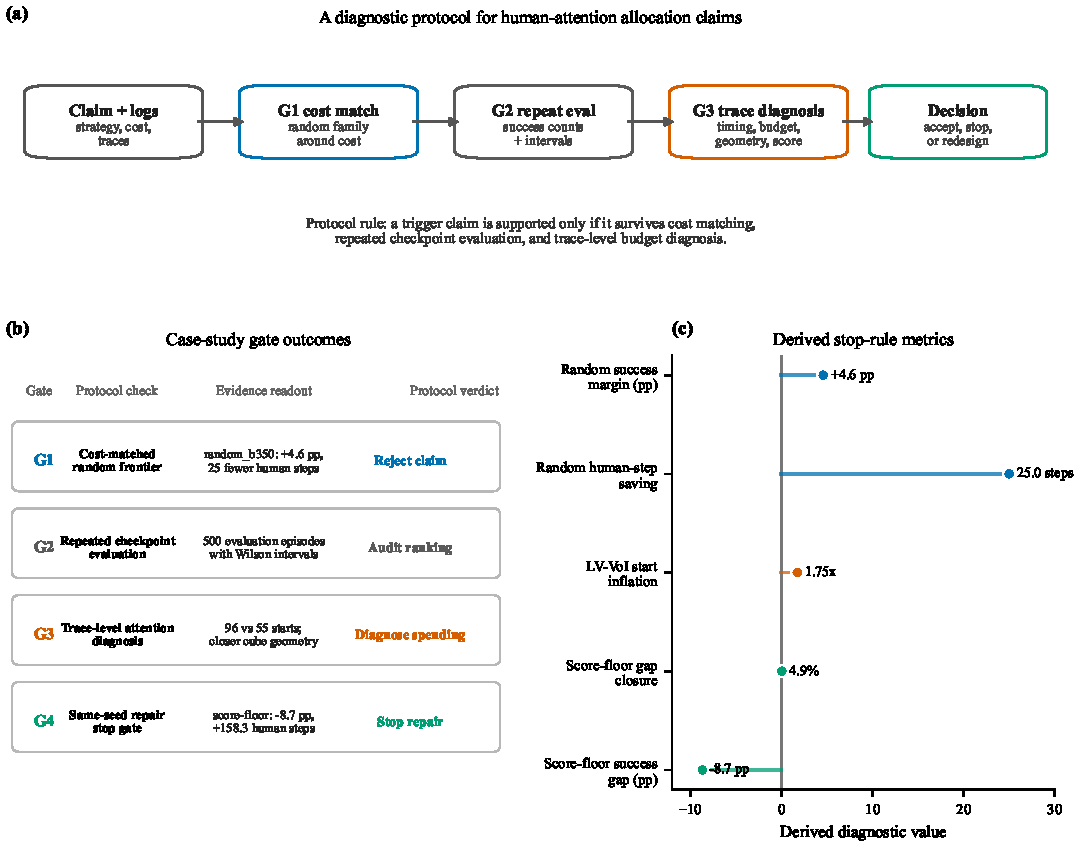
\includegraphics[width=0.95\textwidth]{fig1_methodology_protocol_r056.pdf}
    \caption{Methodology-first overview of the diagnostic evaluation route. The figure states the gate sequence for HIL-RL human-attention allocation claims, then shows the current Lift verdicts and derived stop-rule metrics from registered R021/R023/R024 evidence. It is a protocol visualization rather than a new empirical result.}
    \label{fig:protocol_hero}
\end{figure*}

\begin{table}[t]
\centering
\caption{Registry-generated cost-matched Lift claims. All numeric entries are drawn from the evidence registry.}
\label{tab:registry_costmatched_claims}
\begin{tabular}{llcccc}
\toprule
Strategy & Run & Success & 95\% CI & Human steps & $\Delta$ \\
\midrule
No intervention & R020 & 400/500 = 80.0\% & [76.3, 83.3] & 0.0 & -3.2 pp \\
\textbf{Random b350} & R021 & 439/500 = 87.8\% & [84.6, 90.4] & 177.0 & +4.6 pp \\
LV-VoI scale3 & R021 & 416/500 = 83.2\% & [79.7, 86.2] & 202.0 & +0.0 pp \\
Random b450 & R021 & 426/500 = 85.2\% & [81.8, 88.0] & 250.0 & +2.0 pp \\
Random b600 & R021 & 426/500 = 85.2\% & [81.8, 88.0] & 269.2 & +2.0 pp \\
\bottomrule
\end{tabular}
\end{table}


The reversal is not an artifact of including only one random budget. Random b450 and random b600 provide higher-cost random-family points, while random b350 provides the lower-cost point that invalidates the original efficiency interpretation. This matters because LV-VoI scale3 would look more favorable if it were compared only with the original higher-cost random condition. The result therefore supports the first protocol gate: a human-attention allocation claim should be tested against a local random success-cost frontier, not against a single random baseline selected before the realized method cost is known.

Two lightweight trigger repairs remain negative under the same discipline. The minimum-disagreement repair reached 226/300 repeated successes (75.3\%, 95\% CI [70.2, 79.9]) at 211.7 best-step human steps. The score-floor repair reached 233/300 repeated successes (77.7\%, 95\% CI [72.6, 82.0]) at 253.3 best-step human steps. Both are below the same-seed random b350 reference, which reached 259/300 repeated successes (86.3\%, 95\% CI [82.0, 89.8]) at 95.0 best-step human steps. Table~\ref{tab:registry_trigger_repairs} is generated from the audited registry and is the preferred numeric source for this repair comparison.

\begin{table}[t]
\centering
\caption{Registry-generated negative trigger-repair claims on Lift seeds 0--2.}
\label{tab:registry_trigger_repairs}
\begin{tabular}{llcccc}
\toprule
Strategy & Run & Success & 95\% CI & Human steps & $\Delta$ \\
\midrule
\textbf{Random b350} & R024 & 259/300 = 86.3\% & [82.0, 89.8] & 95.0 & +0.0 pp \\
Min-disagree LV-VoI & R022 & 226/300 = 75.3\% & [70.2, 79.9] & 211.7 & -11.0 pp \\
Score-floor LV-VoI & R024 & 233/300 = 77.7\% & [72.6, 82.0] & 253.3 & -8.7 pp \\
\bottomrule
\end{tabular}
\end{table}


\begin{figure*}[t]
    \centering
    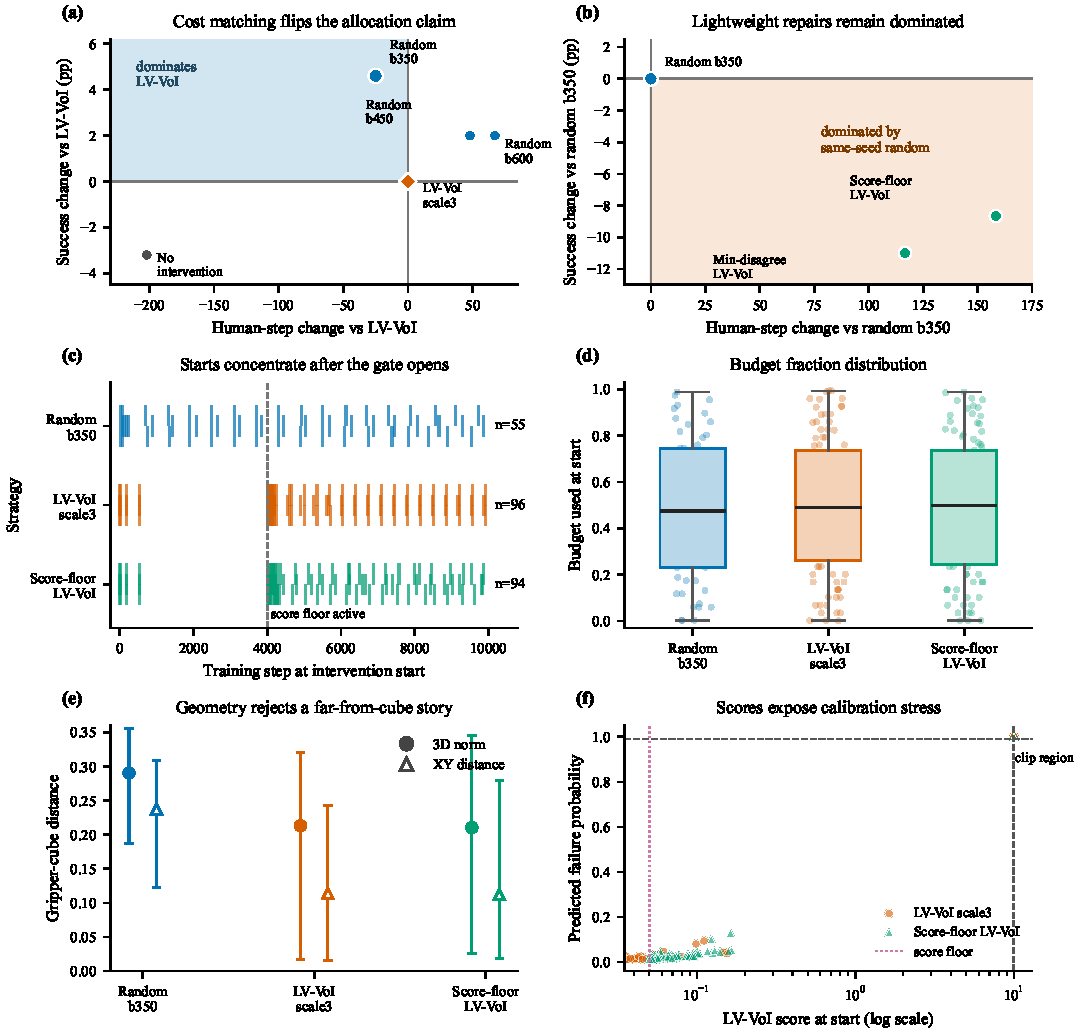
\includegraphics[width=0.95\textwidth]{fig_attention_allocation_diagnostics_r054.pdf}
    \caption{Attention-allocation diagnostics for the current negative trigger result. The panels combine the R021 cost-matched reversal, the R024 repair stop gate, and R023/R024 intervention-start traces to show when budget is spent, how much budget has already been used, where the gripper is relative to the cube, and whether LV-VoI scores or failure probabilities saturate. The figure is diagnostic: it visualizes the registered R021/R023/R024 evidence and does not introduce a new positive method claim.}
    \label{fig:attention_allocation_diagnostics_r054}
\end{figure*}

The trace results sharpen the mechanism claim. Figure~\ref{fig:attention_allocation_diagnostics_r054} summarizes the trace-level evidence without treating it as a new success metric. LV-VoI does not fail merely because it requests interventions far from the cube. In the R023 traces, LV-VoI starts were closer to the cube than random on average, with mean gripper-to-cube norm 0.217 for LV-VoI versus 0.285 for random b350, and mean gripper-to-cube planar distance 0.152 versus 0.235. However, LV-VoI used 96 intervention starts across seeds 0--2 compared with 55 starts for random b350. The trigger therefore appears to spend more budget despite querying in geometrically plausible states, which points away from a simple distance-threshold repair.

The score-floor repair confirms this interpretation. R024 mechanically removed low-score starts after step 4000: the trace table records zero post-floor starts below the 0.05 threshold. Nevertheless, the repair still produced 94 intervention starts, almost the same as the original LV-VoI count of 96 and far above the random b350 count of 55. Its median accepted score was only 0.067, indicating that the floor was too weak to create random-level selectivity. Together, the repair and trace results support a narrower conclusion: the current trigger suffers from budget-control and score-timing mismatch, and any new trigger should be evaluated through the same cost-matched and trace-level protocol before being expanded.

Stack provides boundary evidence rather than a positive generalization result. With a strong matched behavioral-cloning initialization, the no-online-human Stack baseline achieved 131/180 repeated successes (72.8\%) at zero online human cost, while both random intervention and Stack-tuned LV-VoI achieved 107/180 repeated successes (59.4\%) at substantial human cost. These results do not support a broad robotics-transfer claim for the current trigger. They instead reinforce the paper's conservative framing: the Lift evidence motivates the diagnostic protocol, and Stack shows that adding online interventions can be harmful when the task and update mechanism are not aligned.

\section{Discussion}

The case study shows why HIL-RL trigger evaluation should be stricter than a single learned-trigger-versus-random comparison. The original LV-VoI result looked plausible until the random baseline was cost matched. After the random budget sweep, random b350 was both more successful and less expensive than LV-VoI scale3. This reversal is the central empirical lesson of the paper: intervention-trigger quality cannot be judged from nominal budget settings alone, because realized human-step cost determines the relevant comparison. A trigger that appears selective at one baseline budget may be dominated once the random family is placed on the same success-cost axis.

Repeated checkpoint evaluation is the second part of the same discipline. In noisy off-policy robot learning, a final checkpoint or a single restored-best evaluation can make a policy look better or worse than its expected behavior. The current evidence package therefore reports repeated checkpoint success counts and binomial intervals rather than single point estimates. This does not remove all variance, but it makes the uncertainty visible enough to prevent a small or lucky evaluation from carrying a paper-level claim.

The trace analysis is equally important because it changes what kind of repair is justified. The failed trigger was not simply asking far from the object: LV-VoI starts were closer to the cube than random starts, yet they were more frequent and less cost effective. The score-floor repair then showed that a mechanically valid threshold can still fail scientifically if it does not reduce accepted starts enough to recover the frontier. These findings argue against quick heuristic repairs based only on one intuitive failure story. They support a diagnostic workflow in which mechanism hypotheses are checked against start-level timing, geometry, and score distributions before a new trigger is scaled.

The current evidence therefore supports a protocol contribution rather than an algorithmic superiority claim. This distinction is important for a journal-style paper. A dominated trigger result can still be useful when it exposes a systematic evaluation failure mode and turns that failure into a reusable reporting standard. FORESIGHT-HIL should be presented as the audited case study that motivated the protocol, not as a method that currently beats random intervention. The paper's positive contribution is the evaluation discipline: cost-matched random families, repeated checkpoint estimates, trace-level intervention diagnostics, and same-seed stop rules for lightweight repairs.

Several limitations remain. The intervention source is a scripted privileged-state oracle, not a human teleoperator, so the results do not measure real human workload, delay, fatigue, or interface effects. The strongest evidence is concentrated on robosuite Lift, while Stack currently functions as boundary evidence showing that online intervention can underperform a strong no-online baseline. The paper also does not yet provide a redesigned trigger that recovers the success-cost frontier. These limitations should remain explicit because they protect the central claim: before HIL-RL papers claim trigger superiority, they should show that the claim survives cost matching, repeated evaluation, and trace-level budget analysis.

The practical implication is a stop-and-redesign rule. If a trigger variant is dominated by same-seed random on both repeated success and realized human cost, it should not be expanded only because it is intuitively appealing. Future method work should begin from the trace findings rather than from the earlier unsupported superiority story. A stronger trigger may need explicit budget control, calibrated trigger scores, task-phase awareness, or contact-aware intervention logic, but those ideas should enter as new experiments only after the current diagnostic paper spine is stable.

\section{Conclusion}

FORESIGHT-HIL is best supported as a diagnostic evaluation protocol for human-in-the-loop reinforcement learning intervention triggers in robotic manipulation. The current LV-VoI trigger and two lightweight repairs are dominated by cost-matched random baselines, but this negative result is scientifically useful because it exposes how a weaker evaluation could have supported the wrong conclusion. The evidence supports a clear reporting standard: before claiming that an intervention trigger is more human-efficient, HIL-RL studies should compare against cost-matched random families, evaluate selected checkpoints repeatedly, and inspect trace-level budget spending. Future method work should treat these gates as entry requirements rather than as optional post-hoc diagnostics.

\appendix
\section{Reproducibility Inventory}
\label{app:reproducibility_inventory}

The manuscript is organized around a registry-first reproducibility path. Raw run directories under \texttt{results/r0xx\_*} are treated as immutable evidence archives, while paper-facing claims are routed through \texttt{results/EXPERIMENT\_EVIDENCE\_REGISTRY.csv}. This structure is intended to make the diagnostic protocol reproducible without requiring a reader to infer which raw CSV, checkpoint summary, figure script, or prose note supports a claim. Any future rerun should write to a new result directory and receive a new registry row before it is used in the manuscript.

\begin{table*}[t]
\centering
\caption{Reproducibility inventory for the current diagnostic-protocol draft. The entries list the artifact that should be inspected before changing a claim, table, or figure.}
\label{tab:reproducibility_inventory}
\small
\begin{tabular}{p{0.18\textwidth}p{0.30\textwidth}p{0.42\textwidth}}
\toprule
\textbf{Need} & \textbf{Primary artifact} & \textbf{Purpose} \\
\midrule
Claim index & \texttt{results/EXPERIMENT\_EVIDENCE\_REGISTRY.csv} & Machine-readable source for success rates, confidence intervals, human-step costs, paper-artifact decisions, and claim status. \\
Result map & \texttt{results/RESULTS\_INDEX.md} & Human-readable map separating paper-core evidence, historical baselines, and smoke/debug outputs. \\
Numeric audit & \texttt{scripts/audit\_registry\_numbers.py} & Checks registry numbers against primary CSV rows before they are copied into prose, captions, or tables. \\
Source audit & \texttt{scripts/validate\_evidence\_registry.py} & Checks that registry primary sources exist and that CSV sources are readable. \\
Claim tables & \texttt{scripts/generate\_claim\_tables.py} and R036 tables & Regenerates the cost-matched and trigger-repair tables from audited registry rows. \\
Paper-core runs & R020--R024 result directories & Store the Lift cost-matched reversal, negative repairs, and intervention trace diagnostics. \\
Trace schema & \texttt{foresight\_hil/experiments/trace.py} and R023/R024 trace CSVs & Define and record intervention-start timing, budget fraction, geometry, score, and predicted failure diagnostics. \\
Reproduction commands & \texttt{results/r044\_environment\_reproducibility\_audit/REPRODUCTION\_COMMANDS.md} & Central command sheet for smoke checks, verification, and future paper-core rerun planning. \\
Citation contexts & \texttt{paper/CITATION\_AUDIT.md} & Current ledger showing that the manuscript citation contexts were audited without adding unsupported citation keys. \\
\bottomrule
\end{tabular}
\end{table*}

The current local environment audit records Python 3.11.13, robosuite 1.5.2, MuJoCo 3.3.0, Stable-Baselines3 2.3.2, Gymnasium 0.28.1, NumPy 1.26.4, and PyTorch 2.4.0 with CUDA 12.4 available. These versions are sufficient for local smoke checks and registry validation on the audited machine. The same audit also records a known upstream Gym compatibility warning emitted through Stable-Baselines3 imports; the warning does not currently fail the unit test suite.

\begin{table*}[t]
\centering
\caption{Compute and evidence-accounting status for the current paper route. Wall-time accounting for historical paper-core runs is not yet complete and is kept as a pre-submission gap rather than filled retrospectively.}
\label{tab:compute_accounting_status}
\small
\begin{tabular}{p{0.18\textwidth}p{0.25\textwidth}p{0.47\textwidth}}
\toprule
\textbf{Evidence layer} & \textbf{Recorded fields} & \textbf{Remaining pre-submission action} \\
\midrule
Lift main comparison & Seeds, repeated success counts, Wilson intervals, and realized best-step human cost are registered for R020--R021. & Preserve exact rerun commands in a fresh reproduction directory if the full comparison is regenerated. \\
Repair gates & Same-seed seeds 0--2 success, cost, and confidence intervals are registered for R022 and R024. & Keep the negative gate interpretation unless a substantially different mechanism is tested under a new result ID. \\
Trace diagnostics & Intervention-start counts, timing, budget fraction, geometry, score, and predicted failure fields are archived for R023/R024. & Use trace summaries to motivate future methods, but do not treat traces as the primary success-rate evidence. \\
Runtime environment & R044 records package versions, CUDA availability, CLI help checks, and smoke-run outputs. & Add a reviewer-facing environment export or container specification before submission. \\
Version provenance & Project files are organized and audited, but local \texttt{.git} metadata is not recognized as a valid repository. & Repair the repository metadata or create a dated source snapshot before external release. \\
\bottomrule
\end{tabular}
\end{table*}

This inventory is deliberately conservative. It makes missing provenance and historical wall-time accounting visible instead of smoothing them over. The reproducibility claim is therefore limited to the audited registry, command templates, generated tables, and smoke-verified local runtime; it is not a claim that every historical run can be re-created without additional compute or environment setup.

\begin{thebibliography}{99}

\bibitem{luo2025hilserl}
Jianlan Luo, Charles Xu, Jeffrey Wu, and Sergey Levine.
\newblock Precise and dexterous robotic manipulation via human-in-the-loop reinforcement learning.
\newblock \emph{arXiv preprint arXiv:2410.21845}, 2024.

\bibitem{ball2023rlpd}
Philip J. Ball, Laura Smith, Ilya Kostrikov, and Sergey Levine.
\newblock Efficient online reinforcement learning with offline data.
\newblock In \emph{Proceedings of the 40th International Conference on Machine Learning}, PMLR 202:1577--1594, 2023.

\bibitem{retzlaff2024hitl}
Carl Orge Retzlaff, Srijita Das, Christabel Wayllace, Payam Mousavi, Mohammad Afshari, Tianpei Yang, Anna Saranti, Alessa Angerschmid, Matthew E. Taylor, and Andreas Holzinger.
\newblock Human-in-the-loop reinforcement learning: A survey and position on requirements, challenges, and opportunities.
\newblock \emph{Journal of Artificial Intelligence Research}, 79:359--415, 2024.

\bibitem{robosuite2020}
Yuke Zhu, Josiah Wong, Ajay Mandlekar, Roberto Martin-Martin, Abhishek Joshi, Kevin Lin, Abhiram Maddukuri, Soroush Nasiriany, and Yifeng Zhu.
\newblock robosuite: A modular simulation framework and benchmark for robot learning.
\newblock \emph{arXiv preprint arXiv:2009.12293}, 2020.

\bibitem{haarnoja2018sac}
Tuomas Haarnoja, Aurick Zhou, Pieter Abbeel, and Sergey Levine.
\newblock Soft Actor-Critic: Off-policy maximum entropy deep reinforcement learning with a stochastic actor.
\newblock In \emph{Proceedings of the 35th International Conference on Machine Learning}, PMLR 80:1861--1870, 2018.

\bibitem{sac2018applications}
Tuomas Haarnoja, Aurick Zhou, Kristian Hartikainen, George Tucker, Sehoon Ha, Jie Tan, Vikash Kumar, Henry Zhu, Abhishek Gupta, Pieter Abbeel, and Sergey Levine.
\newblock Soft Actor-Critic algorithms and applications.
\newblock \emph{arXiv preprint arXiv:1812.05905}, 2018.

\bibitem{mandlekar2021robomimic}
Ajay Mandlekar, Danfei Xu, Josiah Wong, Soroush Nasiriany, Chen Wang, Rohun Kulkarni, Li Fei-Fei, Silvio Savarese, Yuke Zhu, and Roberto Martin-Martin.
\newblock What matters in learning from offline human demonstrations for robot manipulation.
\newblock In \emph{Proceedings of the 5th Conference on Robot Learning}, PMLR 164:1678--1690, 2022.

\bibitem{hoque2021thrifty}
Ryan Hoque, Ashwin Balakrishna, Ellen Novoseller, Albert Wilcox, Daniel S. Brown, and Ken Goldberg.
\newblock ThriftyDAgger: Budget-aware novelty and risk gating for interactive imitation learning.
\newblock In \emph{Proceedings of the 5th Conference on Robot Learning}, PMLR 164:598--608, 2022.

\bibitem{cai2025aim}
Haoyuan Cai, Zhenghao Peng, and Bolei Zhou.
\newblock Robot-gated interactive imitation learning with adaptive intervention mechanism.
\newblock \emph{arXiv preprint arXiv:2506.09176}, 2025.

\bibitem{chua2018pets}
Kurtland Chua, Roberto Calandra, Rowan McAllister, and Sergey Levine.
\newblock Deep reinforcement learning in a handful of trials using probabilistic dynamics models.
\newblock In \emph{Advances in Neural Information Processing Systems}, 2018.

\bibitem{janner2019mbpo}
Michael Janner, Justin Fu, Marvin Zhang, and Sergey Levine.
\newblock When to trust your model: Model-based policy optimization.
\newblock In \emph{Advances in Neural Information Processing Systems}, 2019.

\bibitem{guo2017calibration}
Chuan Guo, Geoff Pleiss, Yu Sun, and Kilian Q. Weinberger.
\newblock On calibration of modern neural networks.
\newblock In \emph{Proceedings of the 34th International Conference on Machine Learning}, PMLR 70:1321--1330, 2017.

\bibitem{henderson2018deeprlmatters}
Peter Henderson, Riashat Islam, Philip Bachman, Joelle Pineau, Doina Precup, and David Meger.
\newblock Deep reinforcement learning that matters.
\newblock \emph{Proceedings of the AAAI Conference on Artificial Intelligence}, 32(1), 2018.

\bibitem{agarwal2021statisticalprecipice}
Rishabh Agarwal, Max Schwarzer, Pablo Samuel Castro, Aaron Courville, and Marc G. Bellemare.
\newblock Deep reinforcement learning at the edge of the statistical precipice.
\newblock \emph{arXiv preprint arXiv:2108.13264}, 2021.

\bibitem{wilson1927score}
Edwin B. Wilson.
\newblock Probable inference, the law of succession, and statistical inference.
\newblock \emph{Journal of the American Statistical Association}, 22(158):209--212, 1927.

\end{thebibliography}


\end{document}
